\section{System Framework}

\begin{figure}
\centering
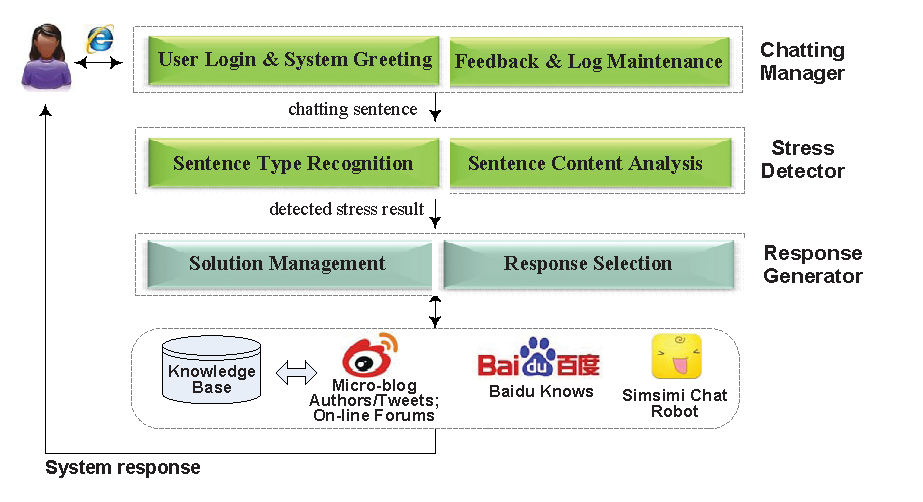
\includegraphics[height=4.9cm]{figs/TeenChatterFramework.eps}
\caption{\emph{TeenChat} framework}
\label{fig:framework}
\end{figure}

\emph{TeenChat} works under the Browser/Server mode. Fig.~\ref{fig:framework} shows its
framework. The user chats with \emph{TeenChat} via an Internet browser.
The \emph{TeenChat} server is comprised of three major components,
which cooperate as follows.
\begin{itemize}
\item \textbf{Chatting Manager}. After a user logins to the system, the \emph{User Login}\&\emph{Sys}
\emph{tem Greeting} module
sends a warm greeting to the user based on the historically detected stress result.
If no historic stress is detected, \emph{TeenChat} will send a greeting like a virtual friend
``\emph{Hello, how��s doing?}", or ``\emph{Is everything ok now}?".
if the user had some stress being detected through previous conversations,
The \emph{Feedback}\&\emph{Log Maintenance} module maintains and refreshes the detected stress result, and adjusts the response
strategy based on feedback analysis (i.e., whether the chatting lasts long, whether the answers
is effective to alleviate user's stress, etc.)

\item \textbf{Stress Detector}.
To understand user's expected answer from the system, the \emph{Sentence Type Recognition} module
categorizes user's chatting sentence into \emph{interrogative question}, \emph{rhetorical question}, or \emph{declarative sentence}.
An interrogative question sentence like ``\emph{How to improve
maths?}" or \emph{What shall I do?}" may ask for objective or positive answers/suggestions,
while a rhetorical question sentence like ``\emph{They should know me, shouldn't they?}"
may reflect user's certain emotions to some extent.
Furthermore, the \emph{Sentence Content Analysis} module senses user's possible stress, including stress category and stress subcategory,
based on the seven adolescent's stress-related lexicons.
If the user's stress is sensed but no stress category/subcategory can be detected
from the current chatting sentence, the previous or historic stress category/subcategory (if available) is assumed as the current stress category/subcategory.
The working of the \emph{Sentence Content Analysis} module is detailed in the next section.


\item  \textbf{Response Generation}.
Based on the stress detection result as well as the chatting sentence type, the
\emph{Response Selection} module chooses an appropriate answer from the local Knowledge Base, Baidu Knows,
or the existing chatting robot Simsimi Repository~\cite{30SIMSIMI}.
The aim is to help stressful users shift attention or express inner struggling, thus
easing the pressure.
The \emph{Solution Management} module is responsible for setting up \emph{TeenChat}'s response strategies during chatting,
and pre-storing a large volume of positive answering sentences in
a local knowledge base, to be managed and incrementally populated
by crawling from on-line forums and influential micro-blog authors/tweets.
\end{itemize}
